\documentclass{article}
\usepackage[utf8]{inputenc}
\usepackage{polski}
\usepackage{geometry}
\usepackage{pdfpages}
\usepackage{pdfpages}
\usepackage{listings}
\usepackage{listingsutf8}
\usepackage{multirow}
\usepackage{siunitx}
\usepackage{multirow}
\usepackage{booktabs}
\usepackage{tabularx}
\usepackage{placeins}
\usepackage{pdflscape}
\usepackage{graphicx}
\usepackage{subfig}
\usepackage{hyperref}
\usepackage{amsmath}
\usepackage{colortbl}

\geometry{
a4paper,
total={170mm,257mm},
left=20mm,
top=20mm
}
\newcolumntype{Y}{>{\centering\arraybackslash}X}
\renewcommand\thesection{}
\lstset{%
literate=%
 {ą}{{\k{a}}}1
 {ę}{{\k{e}}}1
 {Ą}{{\k{A}}}1
 {Ę}{{\k{E}}}1
 {ś}{{\'{s}}}1
 {Ś}{{\'{S}}}1
 {ź}{{\'{z}}}1
 {Ź}{{\'{Z}}}1
 {ń}{{\'{n}}}1
 {Ń}{{\'{N}}}1
 {ć}{{\'{c}}}1
 {Ć}{{\'{C}}}1
 {ó}{{\'{o}}}1
 {Ó}{{\'{O}}}1
 {ż}{{\.{z}}}1
 {Ż}{{\.{Z}}}1
 {ł}{{\l{}}}1
 {Ł}{{\l{}}}1
}

\title{Metody Obliczeniowe w Nauce i Technice\\ 
Laboratorium II}
\author{Maciej Trątnowiecki}
\date{AGH, Semestr Letni, 2020}

\begin{document}
    \maketitle
    % numpy.linalg.solve, numpy.linalg.lstsq, scipy.linalg.lu
    \section{Metoda Gaussa-Jordana}
        % Napisz i sprawdź funkcję rozwiązującą układ równań liniowych n × n metodą Gaussa-Jordana. Dla rozmiarów macierzy współczynników większych niż 500 × 500 porównaj czasy działania zaimplementowanej funkcji z czasami uzyskanymi dla wybranych funkcji bibliotecznych.
        W ramach rozwiązania zadania zaimplementowałem funkcję rozwiązującą układ równań liniowych metodą Gaussa-Jordana. Zastosowałem normalizację (skalowanie) wartości wierszy i częściowe poszukiwanie elementu wiodącego. Otrzymałem rozwiązanie zwracające poprawne wyniki dla testowanych losowych macierzach. Jednakże moja implementacja w pythonie nie jest równie wydajna co choćby biblioteczna funkcja z pakietu numpy. Dla macierzy o rozmiarach nxn wykonałem pomiary czasu wykonania, otrzymując następujące wyniki. 
        \begin{center}
        \begin{tabular}{|c|c|c|c|}
            \hline
             n & Czas numpy & Mój czas & Mój czas jako procent numpy\\
             \hline
             500 & 0.0716 & 2.5172 & 3516\% \\
             \hline
             1000 & 0.0689 & 7.6921  & 11164\% \\
             \hline
             2000 & 0.1845 & 38.7065  & 20979\% \\
             \hline
        \end{tabular}
        \end{center}\\
        
        Różnica jest zatrważająca, nie jest to jednak dużym zaskoczeniem. Funkcje z pakietu numpy z natury są wydajniejsze od zwykłych funkcji pythonowych. Postanowiłem jednak zbadać wzrost czasu potrzebnego na wykonanie obliczeń w zależności od liczby elementów. Otrzymane wartości znormalizowałem, by móc porównać tempo wzrostu.\\
        \begin{figure}[h!]
            \centering
            \subfloat[]{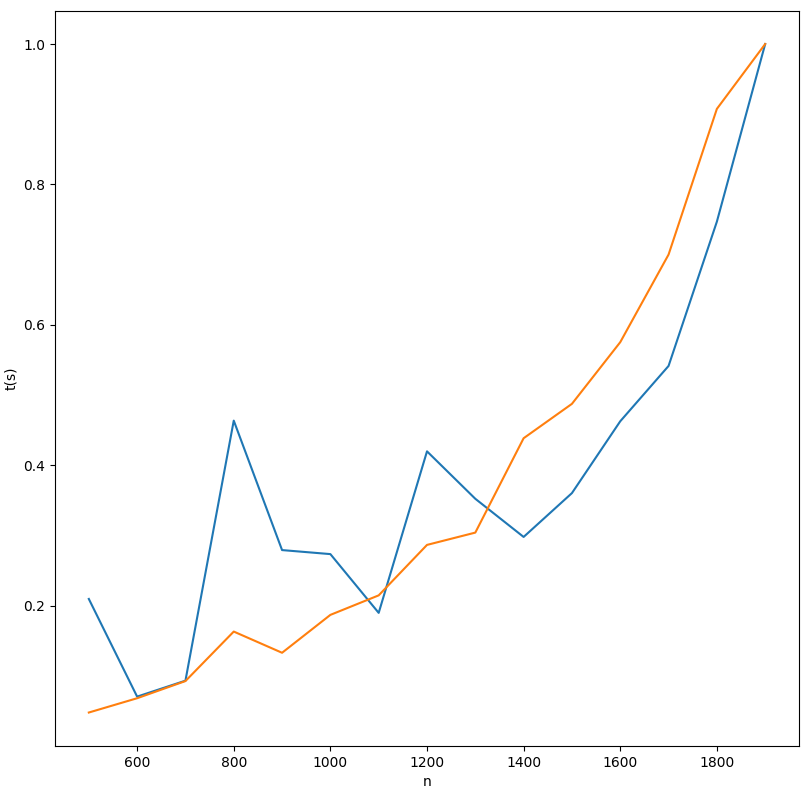
\includegraphics[width=9cm]{lab2/img/time.png}}
            \caption{Wykres zależności czasu wykonania od rozmiaru układu.}
        \end{figure}\\
        Otrzymana zależność sugeruje, że oba algorytmy działają w porównywalnej złożoności obliczeniowej, różnią się za to zdecydowanie w czasach wykonania.\\
        
    \section{Faktoryzacja LU}
        % Napisz i sprawdź funkcję dokonującą faktoryzacji A = LU macierzy A. Zastosuj częściowe poszukiwanie elementu wiodącego oraz skalowanie.
        Następnie przygotowałem implementację prostej faktoryzacji LU macierzy, korzystając z algorytmu Gaussa. Zastosowałem przygotowaną wcześniej normalizację macierzy i częściowe poszukiwanie elementu wiodącego. Poprawność faktoryzacji sprawdziłem mnożąc ze sobą wynikowe macierze L i U. 
         
        
    \section{Analiza obwodu elektrycznego}
        Przygotowałem program analizujący natężenie prądu przepływającego w zadanym obwodzie elektrycznym. Obwód przyjmuje jako graf ważony, nieskierowany o wagach krawędzi oznaczających ich rezystancję. Dodatkowo w grafie wyróżnione zostały dwa węzły, pomiędzy którymi przyłożono znaną siłę elektromotoryczną. \\
        Wynikiem analizy natężeń jest ważony graf skierowany, gdzie wagami krawędzi są natężenia płynącego nimi prądu. Dodatkowo w węzłach grafu oznaczam jego napięcie względem wierzchołka źródłowego.\\
        Do implementacji programu wykorzystałem bibliotekę \textit{networkx}, reprezentując powyżej określone struktury jako pochodne klas \textit{nx.Graph} i \textit{nx.DiGraph}. Dodatkowo przygotowałem wizualizację obu grafów przy wykorzystaniu biblioteki \textit{matplotlib}. W analizie natężeń wykorzystałem także funkcję \textit{numpy.linalg.solve} odpowiadającą za rozwiązanie układu równań liniowych.\\
        Zaimplementowałem także funkcję sprawdzającą poprawność uzyskanych wyników. Za poprawny uznaje się graf wynikowy, w którym suma natężeń prądów wychodzących z węzła, jest równa sumie natężeń prądów wchodzących. \\
        Program umożliwia wczytanie układu z pliku, lub wygenerowanie losowego przykładu. Przygotowałem zbiór przykładowych układów dla celów testowych, znajdujących się w folderze graphs. Funkcja losująca umożliwia wybór typu generowanego grafu, w tym graf regularny i graf z pojedynczym mostkiem. Ze względu na wydajność funkcji generującej wizualizację, dla grafów o dużej liczbie wierzchołków (rzędu kilku tysięcy) warto ograniczyć się do sprawdzenia poprawności wyniku. \\
        
        
        
        
        


    
\end{document}